\documentclass[poly]{mesCours}

\title{Propriétés de fonctions}
\author{Seconde 9}
\date{18 Mars 2024}

\begin{document}
\maketitle
\paragraph{Rappels}
Soit $\function{f}{[-1;4]}{\R}{x}{3x + 1}$.
\begin{enumerate}[label=\alph*)]
\item Quel est l'ensemble de définition de $f$ ?
\item Quelle est l'image de $3$ par $f$ ?
\item $1$ est-il un antécédant de $4$ par $f$ ?
\end{enumerate}
\section{Variation de fonction}
\subsection{Monotonie}
\begin{definition}
Une fonction $f$ est \emph{croissante} sur un intervalle $I$ si la fonction est définie sur $I$, et si, pour tout $x \leq y$ dans $I$, on a
\begin{equation*}
f(x) \leq f(y)
\end{equation*}
Une fonction $f$ est \emph{décroissante} sur un intervalle $I$ si la fonction est définie sur $I$, et si, pour tout $x \leq y$ dans $I$, on a
\begin{equation*}
f(y) \leq f(x)
\end{equation*}
\end{definition}
\begin{remark}
\begin{itemize}
\item Dire d'une fonction qu'elle est croissante ou décroissante, c'est dire qu'elle est croissante ou décroissante sur son ensemble de définition. 
\item On dit d'une fonction croissante qu'elle \emph{conserve l'ordre}; tandis qu'une fonction décroissante \emph{inverse l'ordre}.
\end{itemize}
\end{remark}
\begin{example}
Soit trois fonctions $f$, $g$, $h$, dont l'ensemble de définition est $[0;8]$. Les trois fonctions ont pour courbes représentatives $\mathcal{C}_f$, $\mathcal{C}_g$ et $\mathcal{C}_h$. Compléter les figures ci-dessous pour déterminer si les fonctions $f$, $g$ et $h$ sont croissantes ou décroissantes.
\begin{center}
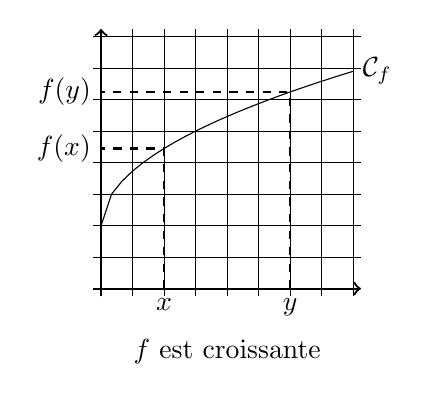
\begin{tikzpicture}[scale=0.4]
\draw[very thin] (-0.25,-0.25) grid (8.25,8.25);
\draw[->,thick] (-0.25,0) -- (8.25,0);
\draw[->,thick] (0,-0.25) -- (0,8.25);
\draw [domain=0:8] plot (\x, {sqrt(3*\x) + 2}) node[right] {$\mathcal{C}_f$};
\draw[dashed,thick] (2,0) node[below] {$x$} -- (2,{sqrt(3*2) + 2}) -- (0, {sqrt(3*2) + 2}) node[left] {$f(x)$};
\draw[dashed,thick] (6,0) node[below] {$y$} -- (6,{sqrt(3*6) + 2}) -- (0, {sqrt(3*6) + 2}) node[left] {$f(y)$};
\draw (4,-2) node {$f$ est croissante};
\end{tikzpicture}
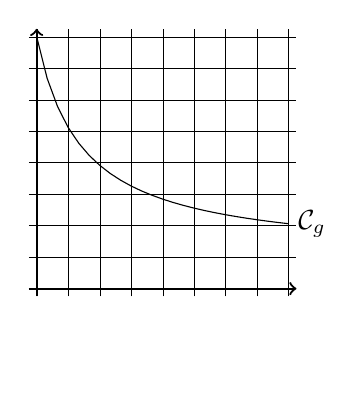
\begin{tikzpicture}[scale=0.4]
\draw[ultra thin] (-0.25,-0.25) grid (8.25,8.25);
\draw[->,thick] (-0.25,0) -- (8.25,0);
\draw[->,thick] (0,-0.25) -- (0,8.25);
\draw[domain=0:8] plot (\x,{1/(0.1*\x + 1/7) + 1}) node[right] {$\mathcal{C}_g$};
\draw (4,-2.5) node {};
\end{tikzpicture}
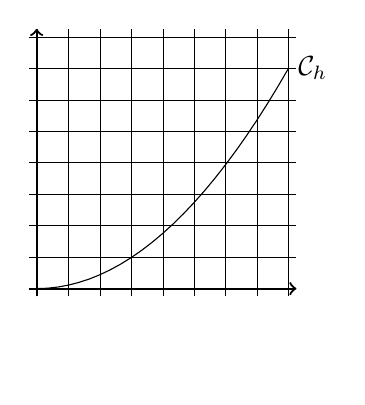
\begin{tikzpicture}[scale=0.4]
\draw[ultra thin] (-0.25,-0.25) grid (8.25,8.25);
\draw[->,thick] (-0.25,0) -- (8.25,0);
\draw[->,thick] (0,-0.25) -- (0,8.25);
\draw[domain=0:8] plot (\x,{(\x * sqrt(7) / 8)^2}) node[right] {$\mathcal{C}_h$};
\draw (4,-2.5) node {};
\end{tikzpicture}
\end{center}
\end{example}
\vspace*{1cm}
Quand une fonction est soit croissante soit décroissante sur un intervalle $I$, on dit que cette fonction est monotone sur cet intervalle $I$.
\paragraph{Demonstrations}
Nous prouvons la croissance de $f : x \mapsto x^2$ et de $g : x \mapsto \sqrt{x}$ sur l'intervalle $\left[0;+\infty\right[$.

\vspace{1cm}
\emptybox{10cm}
\subsection{Tableau de variation}
\begin{center}
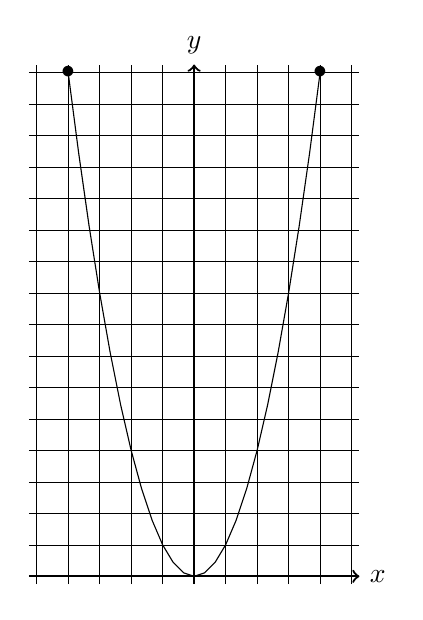
\begin{tikzpicture}[scale=0.4]
\draw[very thin] (-5.25,-0.25) grid (5.25,16.25);
\draw[->,thick] (-5.25,0) -- (5.25,0) node[right] {$x$};
\draw[->,thick] (0,-0.25) -- (0,16.25) node[above] {$y$};
\draw[domain=-4:4] plot (\x,{\x*\x}) node {$\bullet$};
\draw (-4,16) node {$\bullet$};
\end{tikzpicture}
\end{center}
\vspace*{1cm}
Pour étudier les variations d'une fonction, on dresse un \emph{tableau de variation} de cette fonction. Ici, nous étudions la fonction $\function{f}{\left[-4;4\right]}{\R}{x}{x^2}$, dont la courbe représentative est donnée ci-dessus. Alors, la tableau de variation est représenté comme ceci :
\begin{center}
\begin{tikzpicture}
\tkzTabInit{$x$ /0.5, $f(x)$ / 2}{$-4$, $0$, $4$};
\tkzTabVar{+/ $16$, - / $0$, + / $16$ };
\end{tikzpicture}
\end{center}
\begin{example}
Soit $g$ la fonction définie sur $\left]-3;4\right]$ dont la courbe représentative est donnée par :
\begin{center}
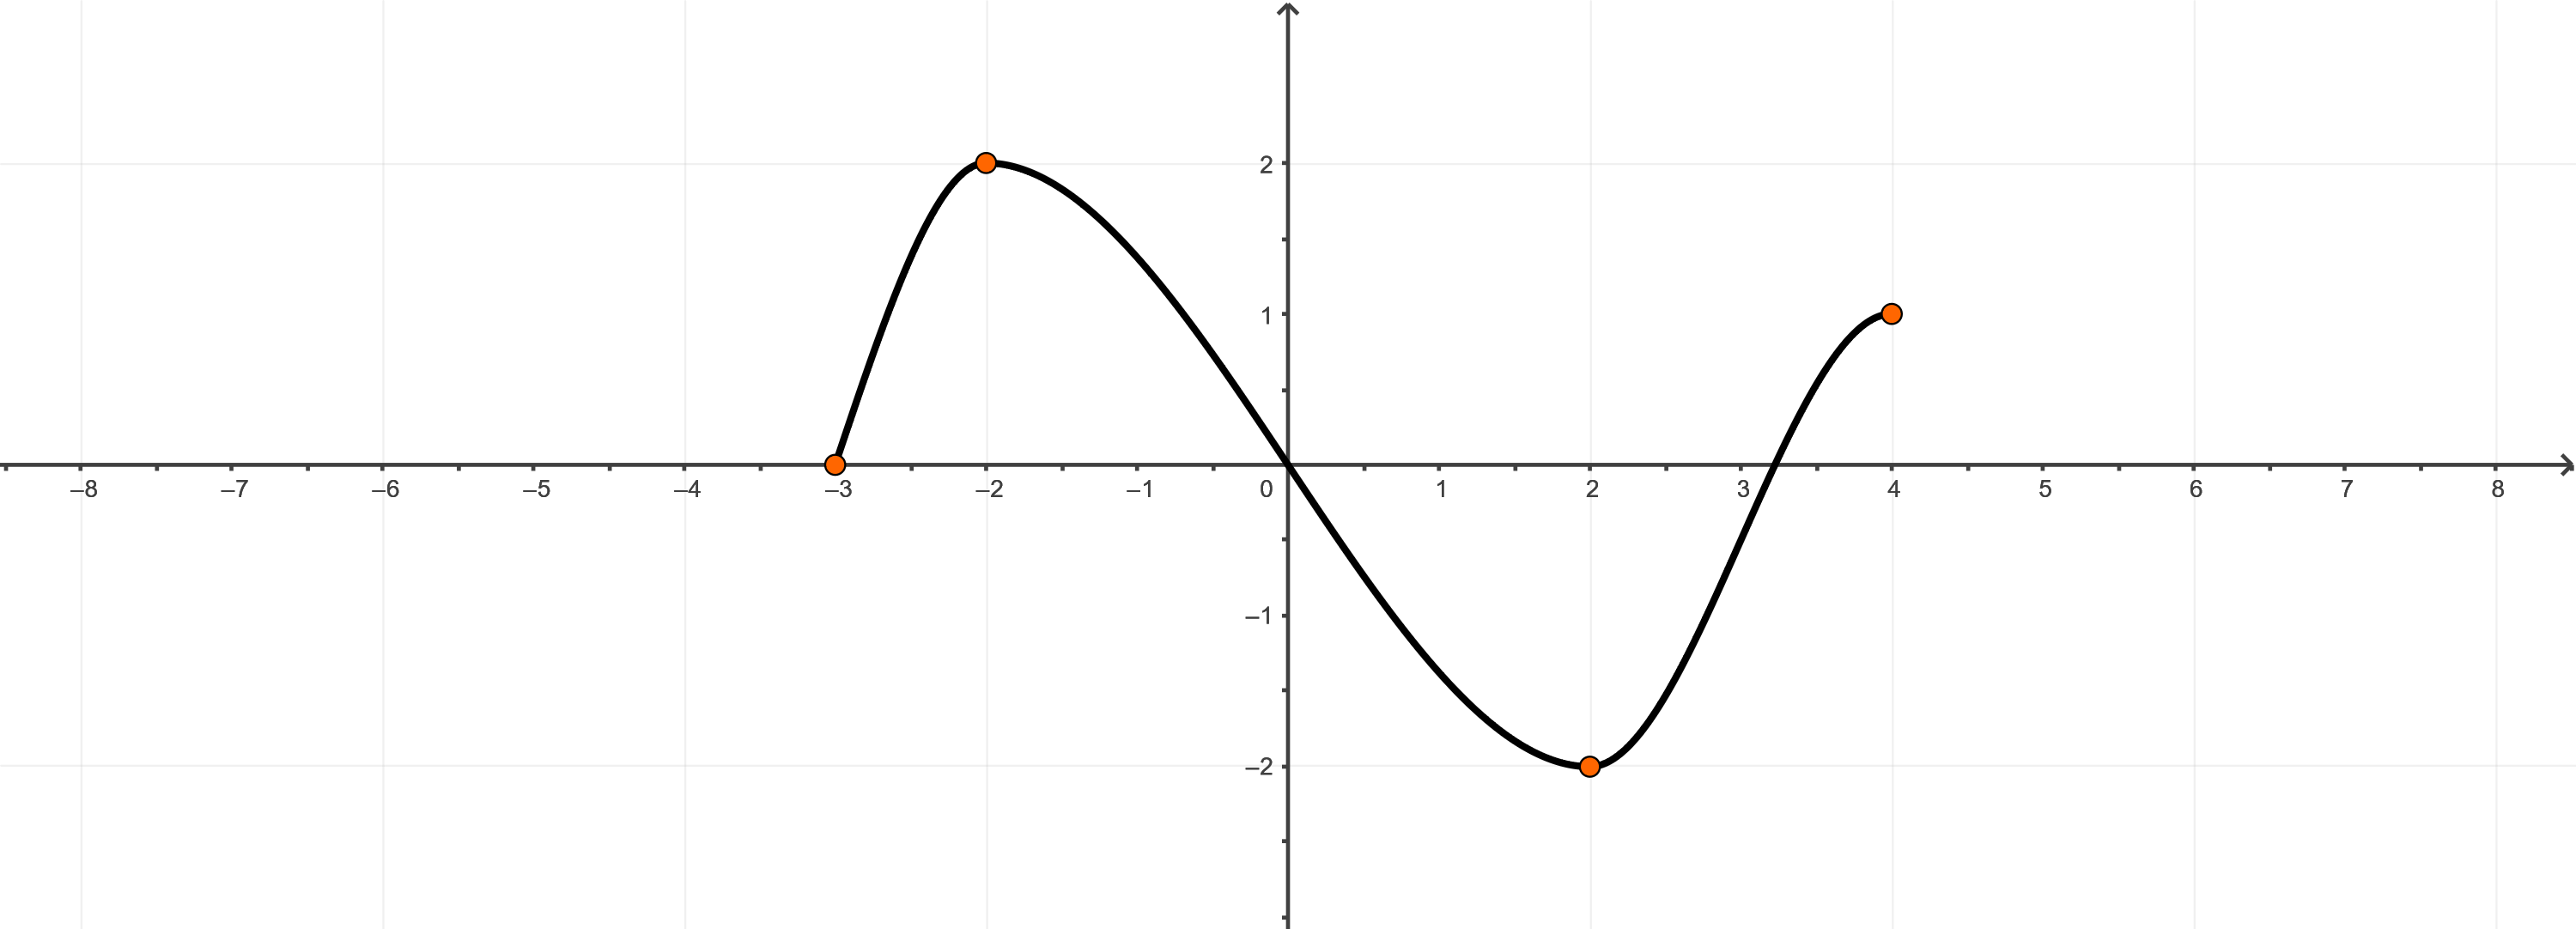
\includegraphics{Polynome1.png}
\end{center}
Compléter son tableau de variation :
\begin{center}
\begin{tikzpicture}
\tkzTabInit{$x$ /0.5, $g(x)$ / 2}{$-3$, $-2$, $2$, $4$}; 
\end{tikzpicture}
\end{center}
\end{example}
\newpage
\begin{example}
La \emph{fonction inverse} est définie comme suit : 
\begin{equation*}
    \function{f}{\left]-\infty;0\right[\cup\left]0;+\infty\right[}{\R}{x}{\dfrac{1}{x}}
\end{equation*}
Cette fonction possède une valeur \og interdite \fg : on ne peut pas diviser par $0$. Voici sa courbe représentative :
\begin{center}
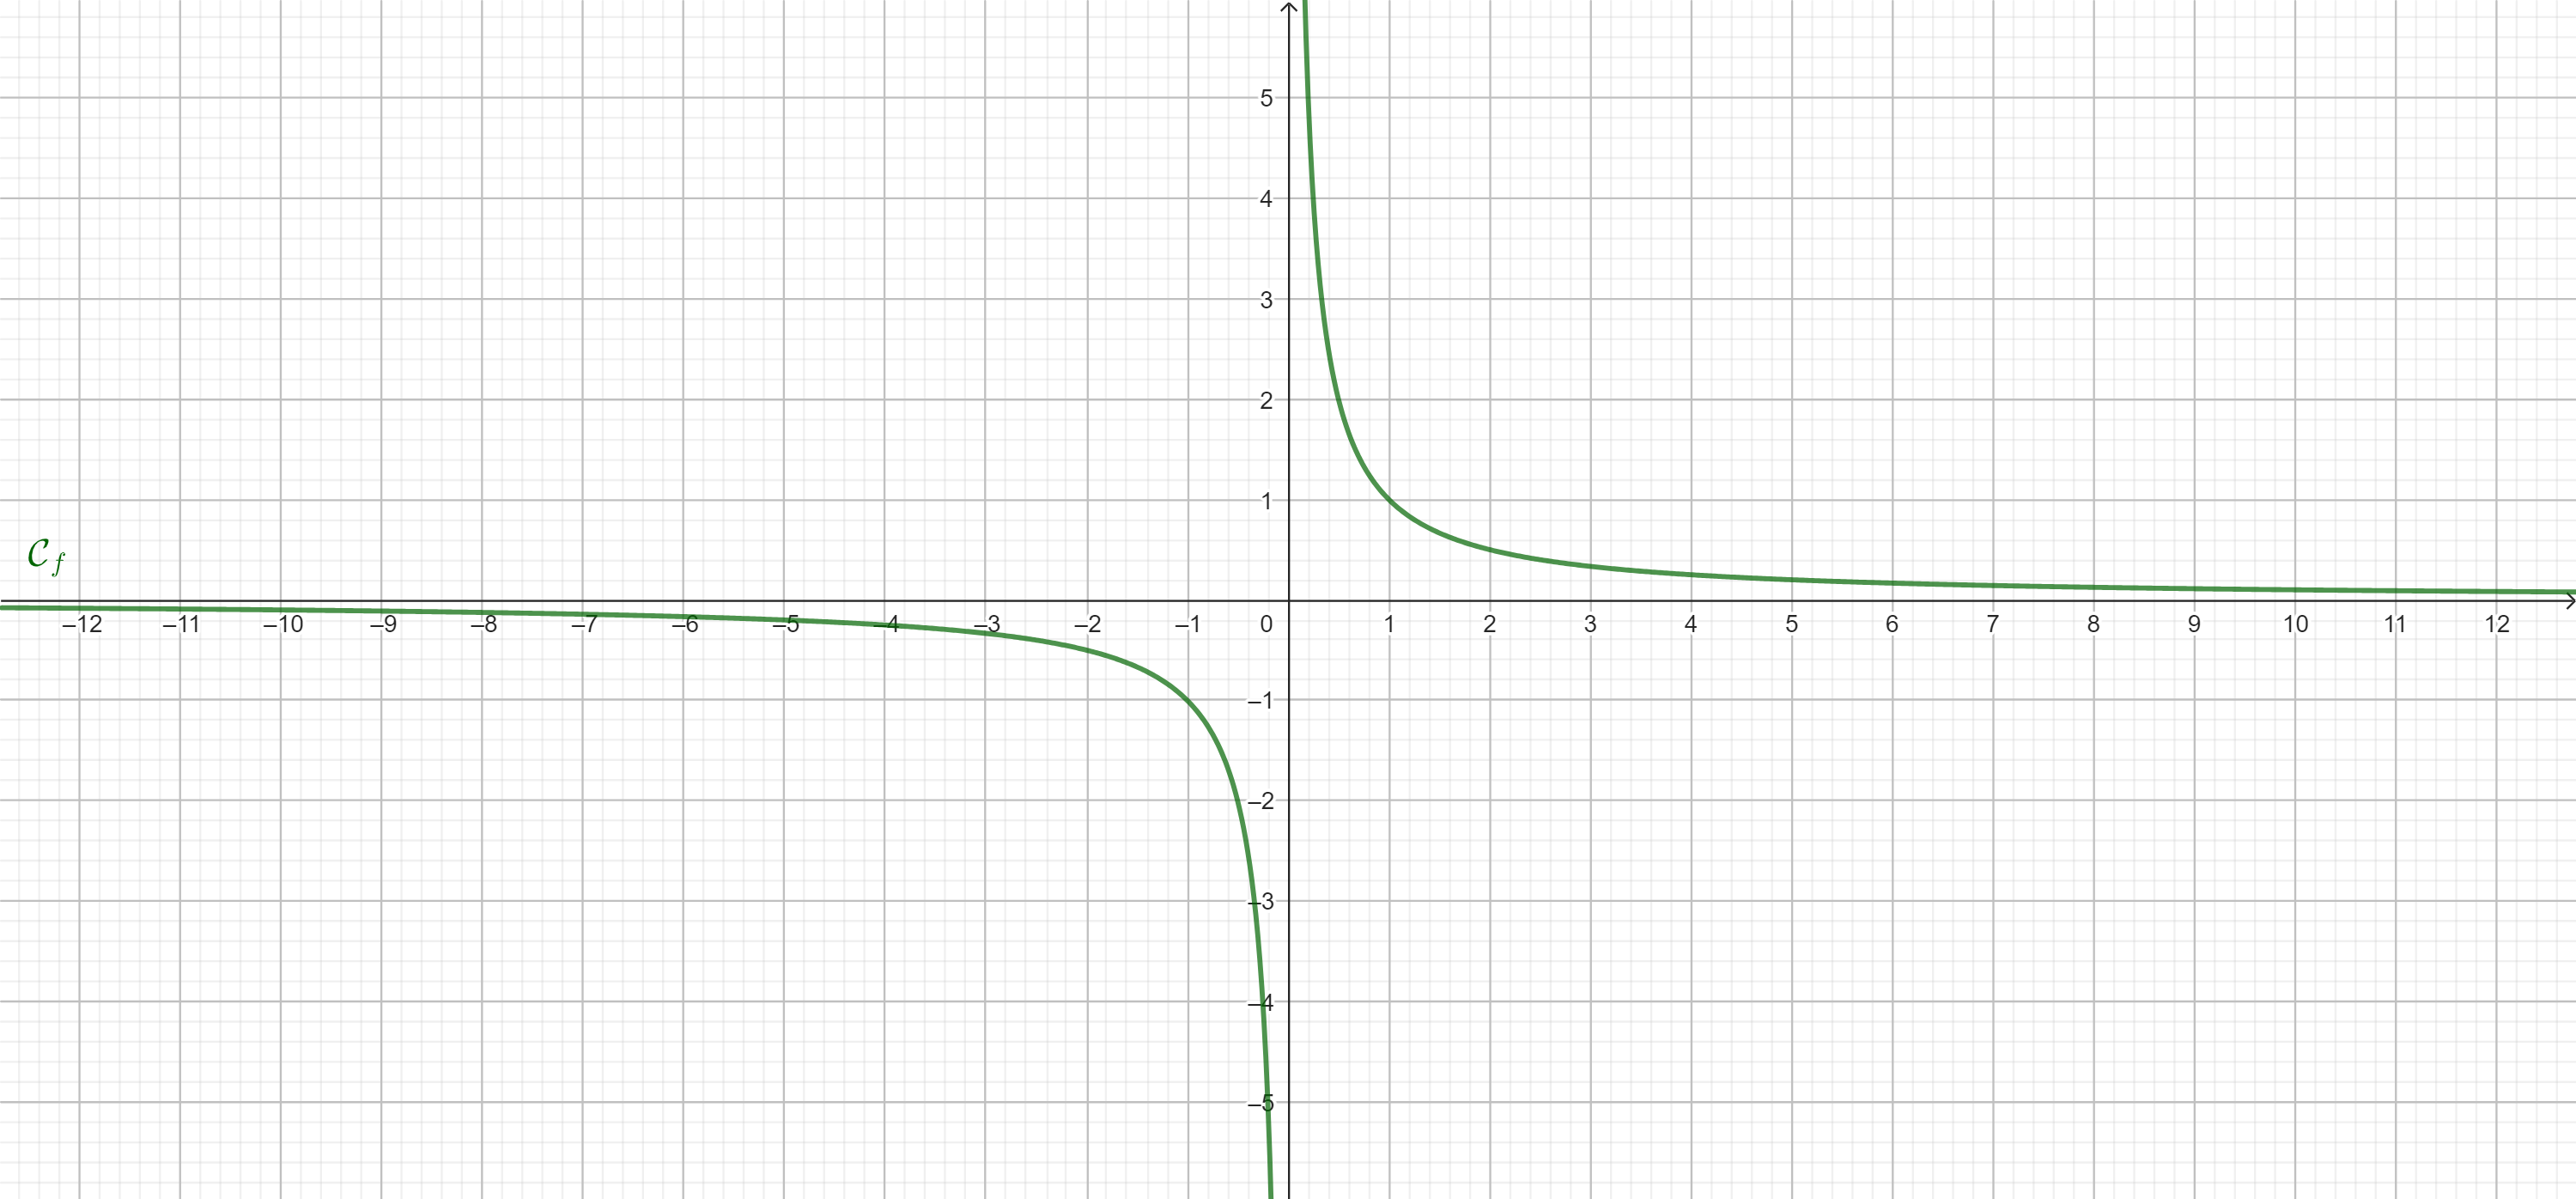
\includegraphics[scale=0.7]{Inverse.png}
\end{center}
L'ensemble de définition de $f$ est donc la réunion d'intervalles $\left]-\infty;0\right[\cup\left]0;+\infty\right[$. Cela se répercute sur le tableau de variation.
\begin{center}
\begin{tikzpicture}
\tkzTabInit{$x$/0.5, $f(x)$/2}{$-\infty$, $0$, $+\infty$};
\tkzTabVar{+/,-D+//,-/};
\end{tikzpicture}
\end{center}
En définitive :
\begin{itemize}
\item La fonction inverse est décroissante sur $\left]-\infty;0\right[$.
\item La fonction inverse est décroissante sur $\left]0;+\infty\right[$.
\end{itemize}
Montrer que la fonction inverse n'est PAS décroissante sur son ensemble de définition.

\vspace*{1cm}
\emptybox{5cm}
\end{example}
\newpage

\section{Extremums}
\begin{definition}
Soit $f$ une fonction à valeurs réelles et $I$ un intervalle sur laquelle $f$ est définie. 
\begin{itemize}
\item La fonction $f$ admet un \emph{maximum} sur $I$ s'il existe $a \in I$ tel que pour tout $x \in I$, $f(x) \leq f(a)$. Dans ce cas, $f(a)$ est le \emph{maximum} de $f$ sur $I$.
\item La fonction $f$ admet un \emph{minimum} sur $I$ s'il existe $b \in I$ tel que pour tout $x \in I$, $f(x) \geq f(b)$. Dans ce cas, $f(b)$ est le \emph{minimum} de $f$ sur $I$.
\end{itemize}
\end{definition}
\begin{remark}
\begin{itemize}
\item Chercher les extremums d'une fonction $f$ sur un intervalle $I$, c'est chercher un maximum $f(a)$ et un minimum $f(b)$ de $f$ avec $a$ et $b$ appartenant à $I$.
\item Le maximum et le minimum d'une fonction $f$ (sans préciser d'intervalle), correspondent aux maximum et minimum de $f$ sur son ensemble de définition.
\end{itemize}
\end{remark}
\begin{example}
Soit $f$ la fonction dont la courbe représentative est donnée ci-après.
\begin{center}
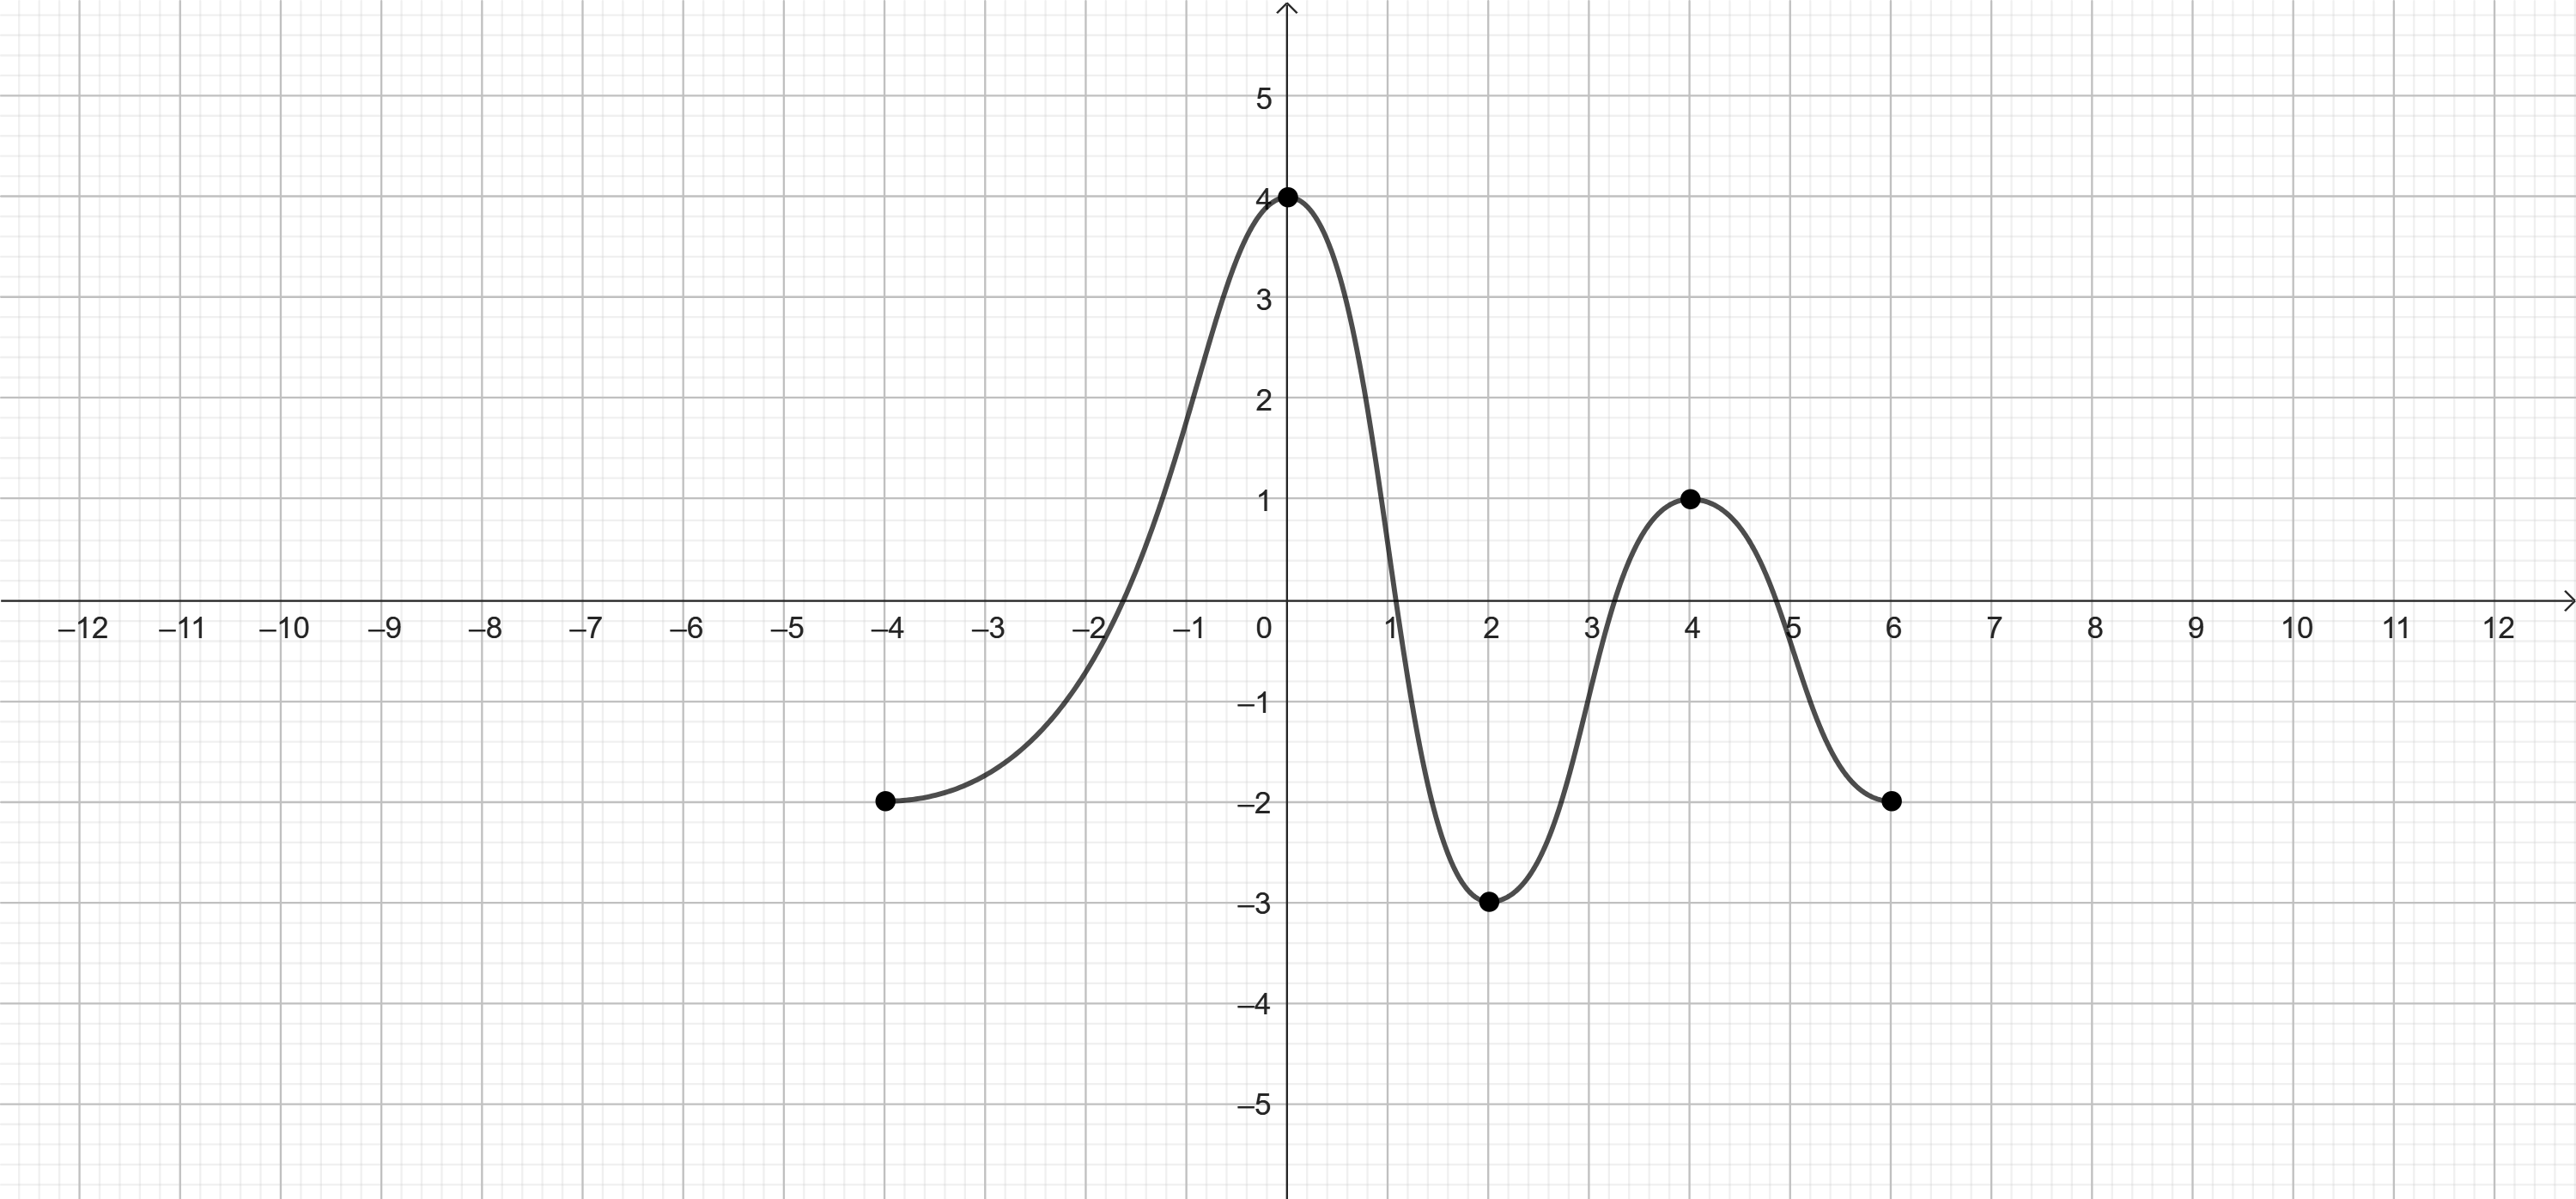
\includegraphics[scale=0.7]{Polynome2MaxMin.png}
\end{center}
\begin{enumerate}
\item Compléter le tableau de variation suivant.
\end{enumerate}
\begin{center}
\begin{tikzpicture}
\tkzTabInit{$x$/0.5, $f(x)$/2}{$-4$ , , , $6$};
\end{tikzpicture}    
\end{center}
\begin{enumerate}[resume*]
\item Quel est le maximum de $f$ ? En quelle valeur ce maximum est-il atteint ? 
\item Quel est le minimum de $f$ ? En quelle valeur ce minimum est-il atteint ? 
\end{enumerate}
\end{example}
\vspace*{1cm}
\emptybox{4cm}

\newpage

\section{Parité d'une fonction}
\subsection*{Fonctions paires}
\begin{definition}
Soit $f$ une fonction définie sur un ensemble $I$ centré en $0$. Une fonction est \emph{paire} si, pour tout $x$ dans $I$, on a
\begin{equation*}
f(-x)=f(x)
\end{equation*}
\end{definition}
\begin{remark}
L'hypothèse \og $I$ est centré en $0$\fg signifie que si $x$ est dans $I$, alors $-x$ est dans $I$. C'est fondamental pour la définition de $f$.
\end{remark}
\begin{example}
On considère la fonction carrée $f : x \mapsto x^2$ définie sur $\R$. Montrer que $f$ est paire.
\end{example}
\vspace*{0.5cm}
\emptybox{3cm}
\subsection*{Fonctions Impaires}
\begin{definition}
Soit $f$ une fonction définie sur un ensemble $I$ centré en $0$. Une fonction est \emph{paire} si, pour tout $x$ dans $I$, on a
\begin{equation*}
f(-x) = -f(x)
\end{equation*}
\end{definition}
\begin{example}
On considère la fonction cube $f : x \mapsto x^3$ définie sur $\R$. Montrer que $f$ est impaire.
\end{example}
\vspace*{0.5cm}
\emptybox{3cm}
\vspace*{0.5cm}
\begin{center}
\begin{minipage}{0.45\textwidth}
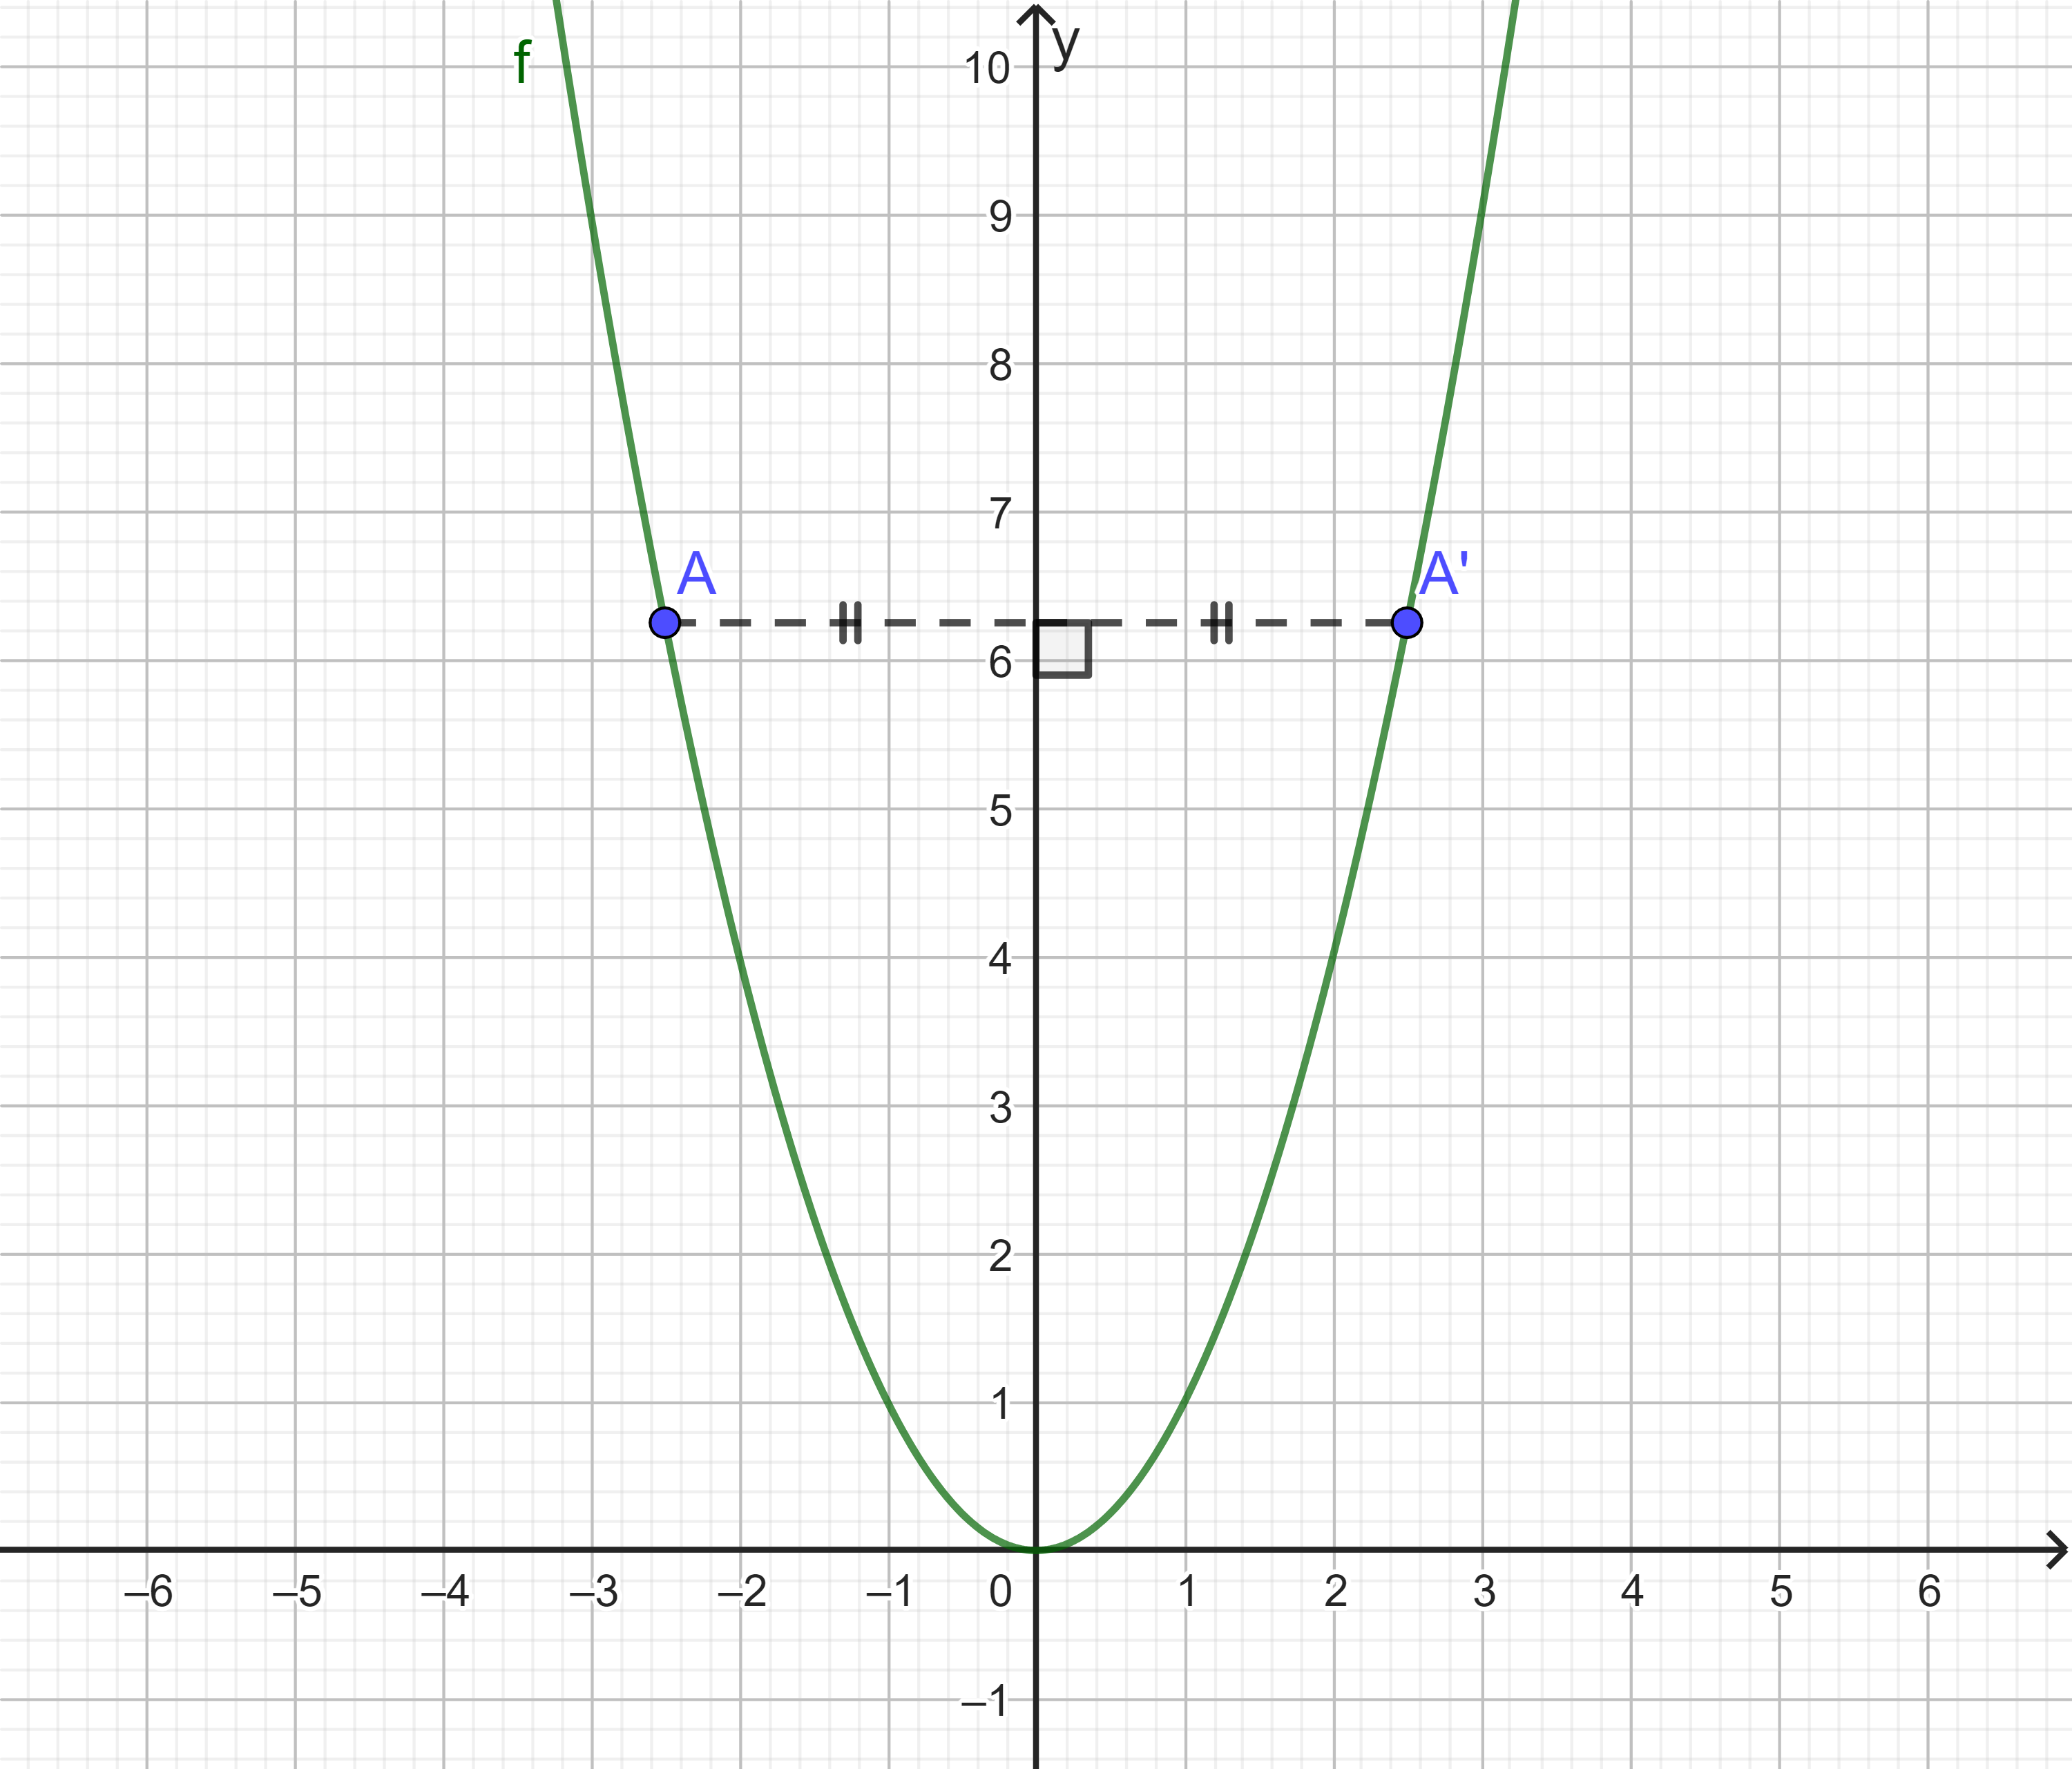
\includegraphics[width=\textwidth]{Carre.png}
La courbe représentative d'une fonction paire est symmétrique par rapport à l'axe des ordonnées.
\end{minipage} \hfill
\begin{minipage}{0.45\textwidth}
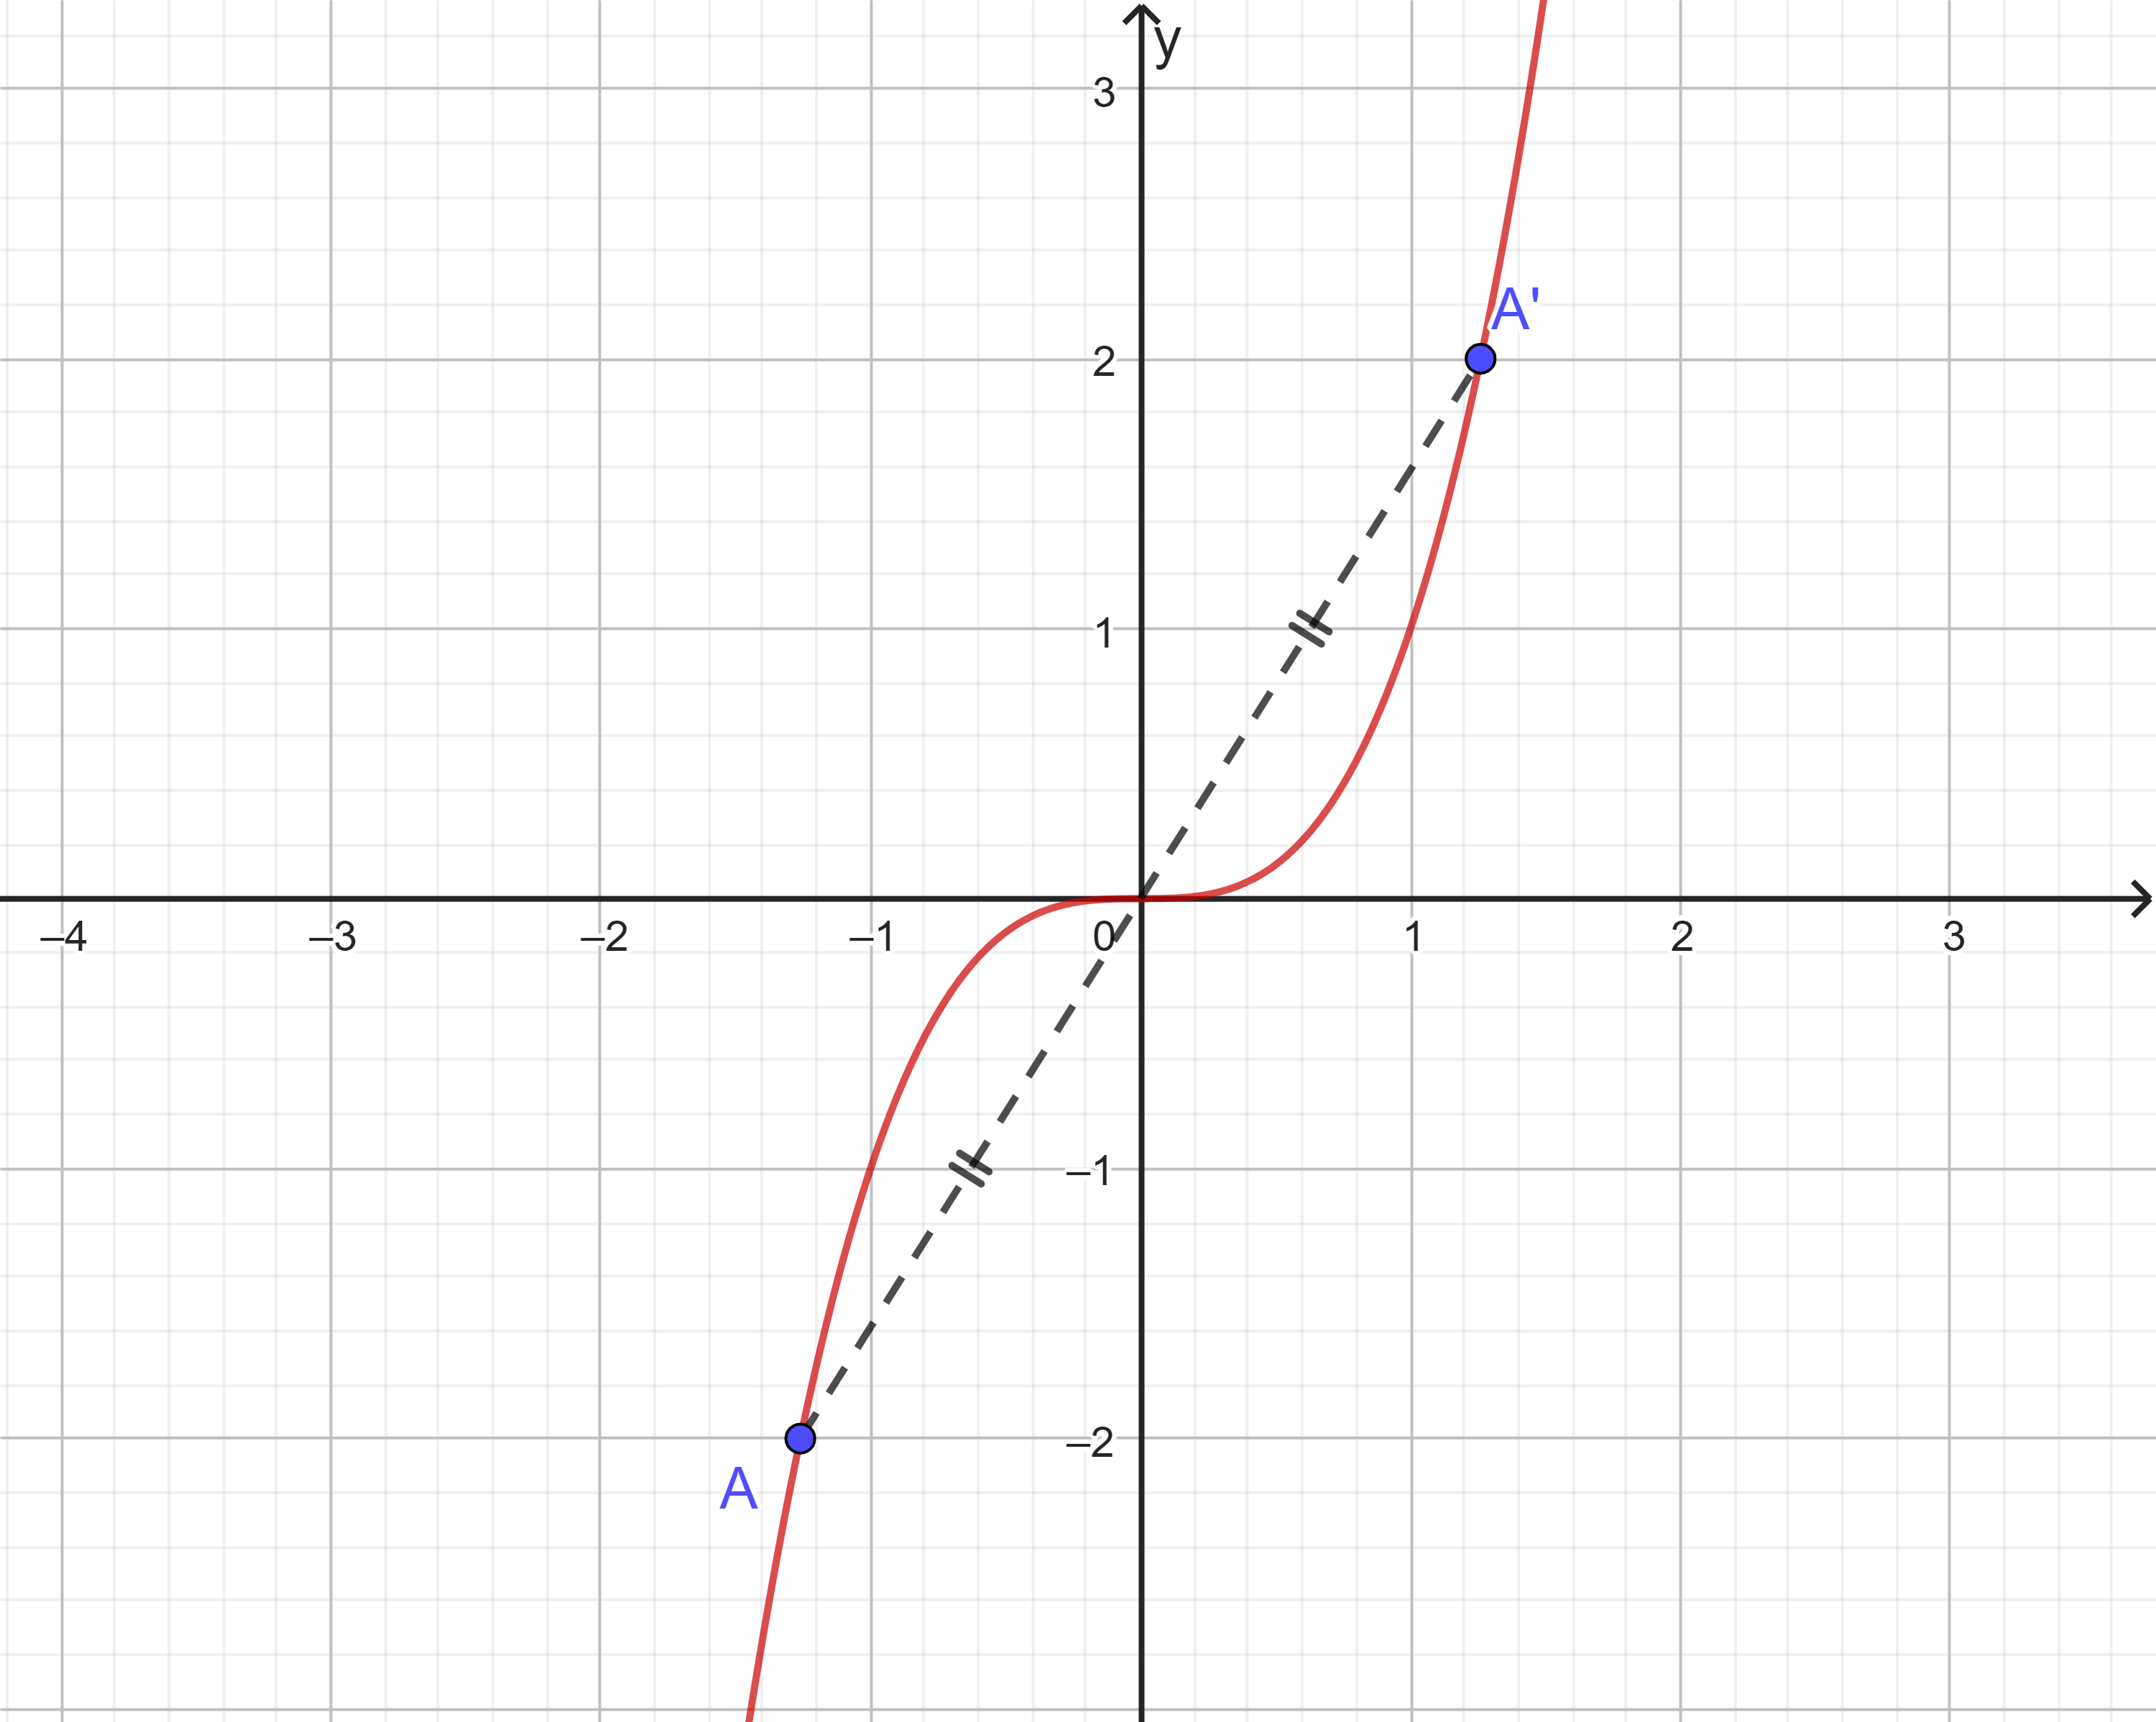
\includegraphics[width=\textwidth]{Cube.png}
La courbe représentative d'une fonction impaire est symmétrique par rapport à l'origine du repère.
\end{minipage}
\end{center}
\newpage
\section{Récapitulatif : étude d'une fonction}
\subsection*{Exemple de fonction}
\begin{equation*}
\function{f}{\left[-2;2\right]}{\R}{x}{-x^3+2x^2+3x+1}
\end{equation*}
\subsection*{Courbe représentative}
\begin{center}
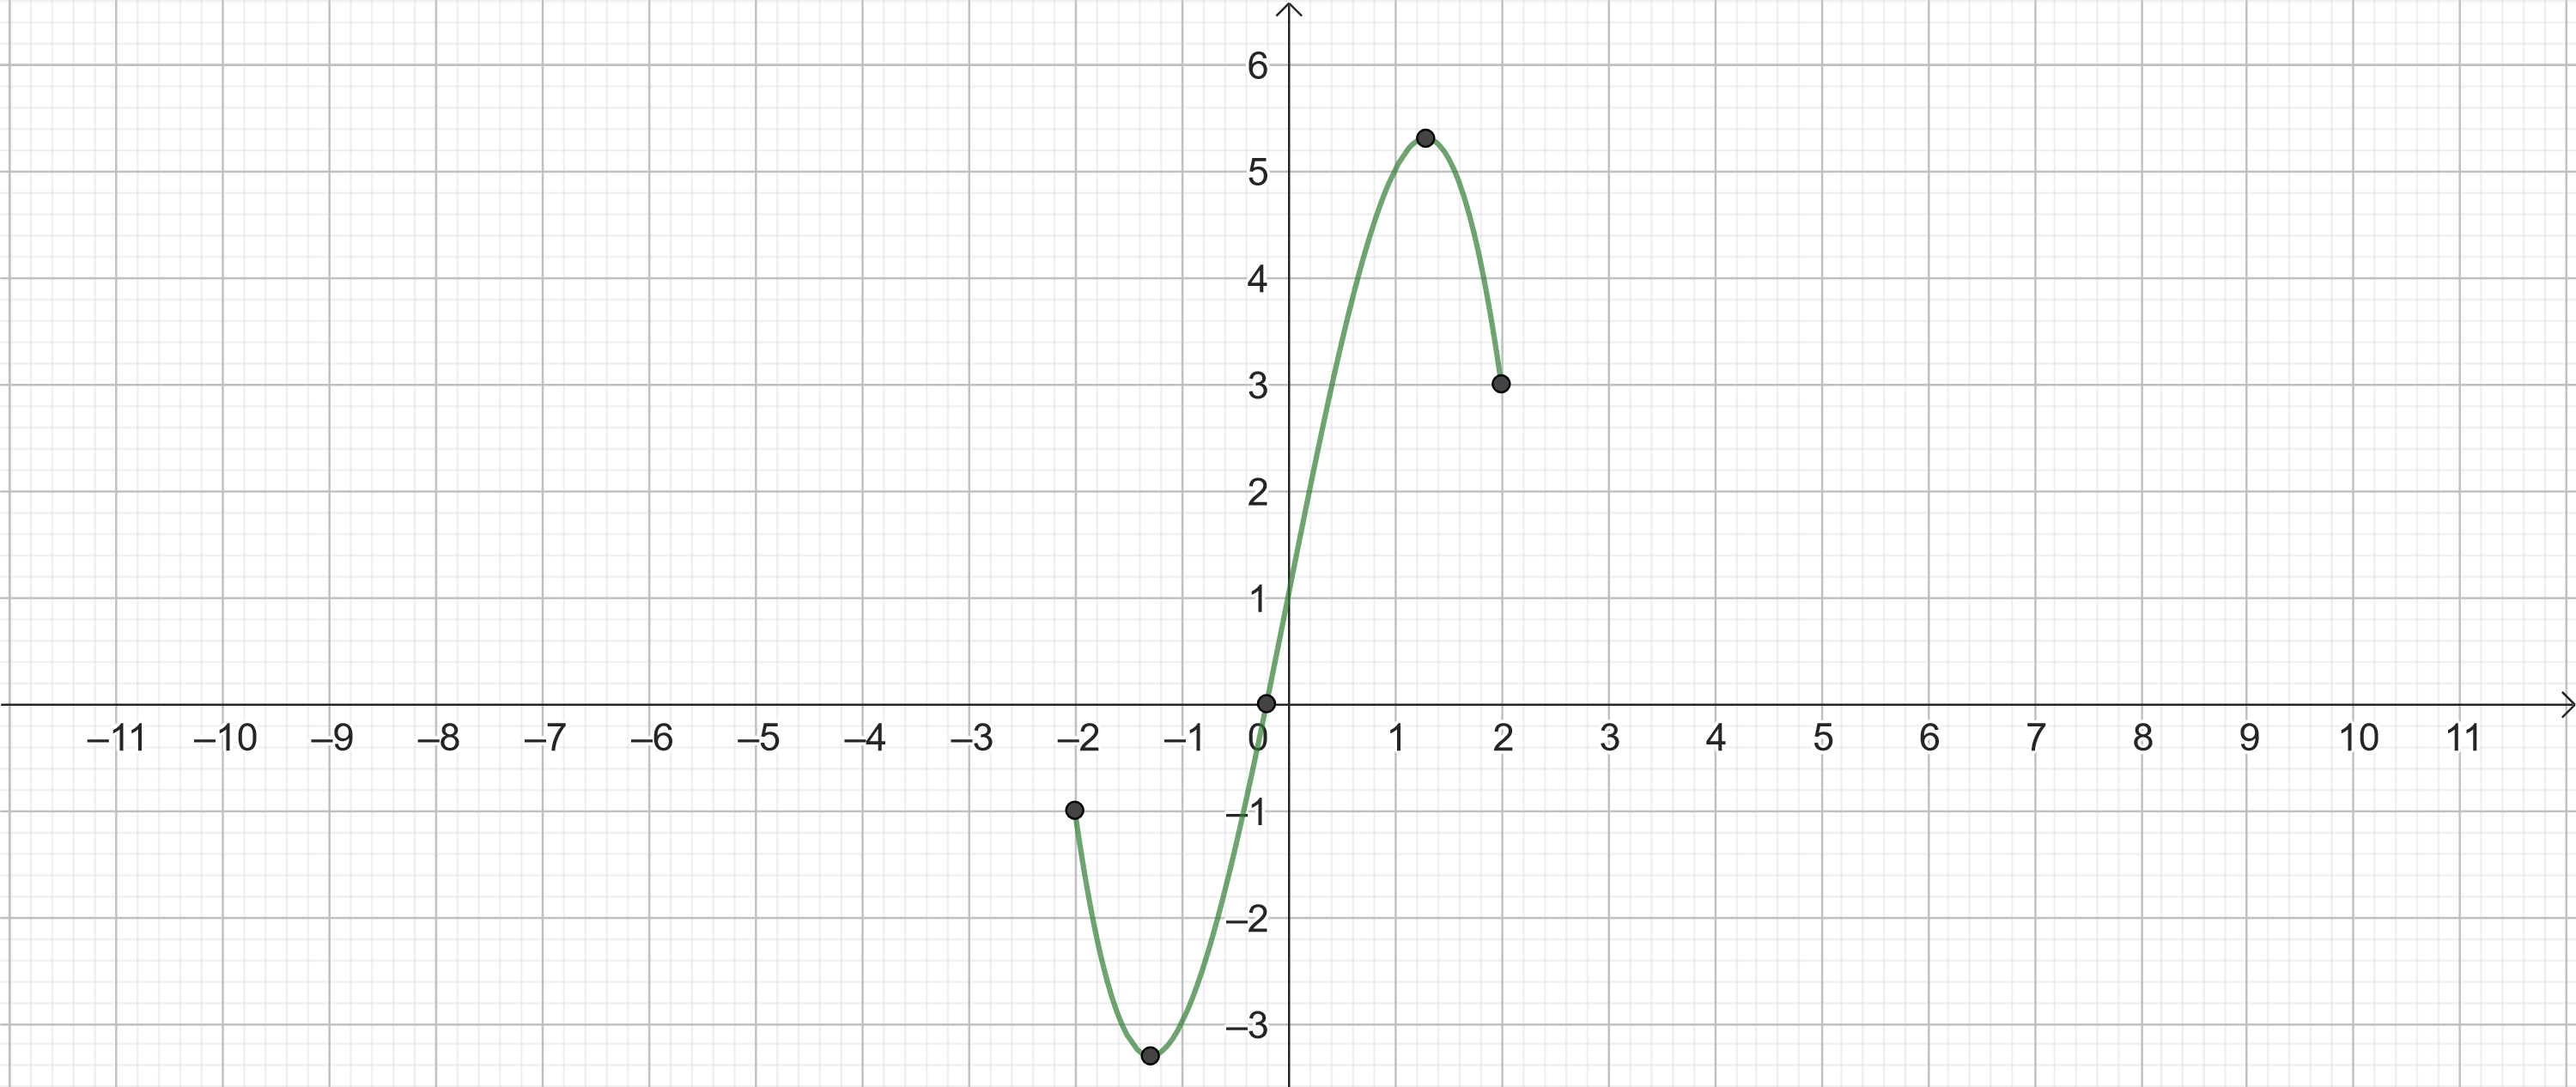
\includegraphics[width=\textwidth]{Recapitulatif.png}
\end{center}
\subsection*{Tableau de valeurs}
Indique l'image par la fonction $f$ de différents antécédants appartenant à l'ensemble de définition de $f$.
\begin{center}
\begin{tikzpicture}
\tkzTabInit{$x$/1, $f(x)$/1}{$-2$, $-1$, $0$, $1$, $2$};
\end{tikzpicture}
\end{center}
\subsection*{Tableau de signes}
Indique le signe d'une fonction, c'est-à-dire les intervalles où la fonction est positive, et les intervalles où la fonction est négative.
\begin{center}
\begin{tikzpicture}
\tkzTabInit{$x$/1,Signe de $f$/1}{$-2$,{$-0,2$},$2$};
\tkzTabLine{ , , z , , };    
\end{tikzpicture}  
\end{center}
\subsection*{Tableau de variations}
Indique les variations de la fonction, c'est-à-dire les intervalles sur lesquelles la fonction est monotone.
\begin{center}
\begin{tikzpicture}
\tkzTabInit{$x$/1,Variations de $f$/2}{$-2$, {$-1,29$},{$1,29$},$2$};
\end{tikzpicture}
\end{center}


\end{document}